
\begin{figure}[H]
  \centering
  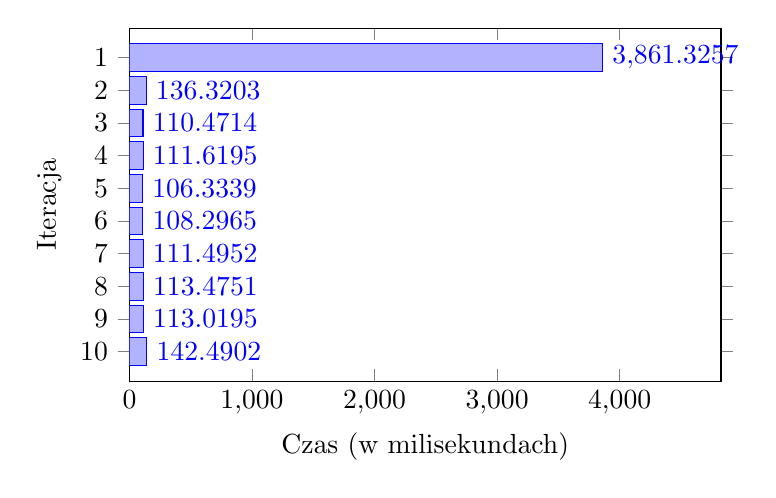
\begin{tikzpicture}
  
    \begin{axis} [
      xbar = .05cm,
      nodes near coords,
      nodes near coords style={
        /pgf/number format/precision=4,
      },
      xmin = 0,
      ytick = data,
      enlarge x limits = {value = .25, upper},
      symbolic y coords = {10,9,8,7,6,5,4,3,2,1},
      xlabel=Czas (w milisekundach),
      ylabel=Iteracja,
      width=0.75\textwidth,
      height=0.5\textwidth
    ]
    
      \addplot coordinates {(3861.325700044632,1) (136.3202999830246,2) (110.47139996290207,3) (111.61949998140335,4) (106.333899974823,5) (108.29649996757507,6) (111.4951999783516,7) (113.47510004043579,8) (113.01950001716614,9) (142.4902000427246,10)};
      
    \end{axis}
  
  \end{tikzpicture}
  \caption{Wynik testów przykładu 8 [\ref{lst:wydajnosc-przyklad-p-8}]}
  \label{fig:wynik-przyklad-7}
\end{figure}
